\documentclass[11pt,a4paper]{article}
\usepackage[utf8]{inputenc}
\usepackage[T1]{fontenc}
\usepackage{lmodern}
\usepackage{geometry}
\usepackage{graphicx}
\usepackage{float}
\usepackage{booktabs}
\usepackage{amsmath}
\usepackage{hyperref}
\geometry{margin=2.2cm}

\title{g4play: Geometrie, běh simulací a NN model PID}
\author{Projektová dokumentace}
\date{\today}

\begin{document}
\maketitle

\section{Model geometrie v Geant4}
Geometrie je implementována v \texttt{src/waterCherenkovSim.cpp}. Sestava obsahuje:
\begin{itemize}
  \item světový objem: box se vzduchem (poloviční rozměry \(3\times3\times4\) m),
  \item válcovou nádrž z nerezu: vnější poloměr \(1{.}75\) m, poloviční výška \(2{.}0\) m,
  \item tloušťku stěny a vík: \(4\) mm,
  \item vnitřní vodní objem: poloměr \(1{.}75\text{ m}-4\text{ mm}\), poloviční výška \(2{.}0\text{ m}-4\text{ mm}\).
\end{itemize}

Optické vlastnosti vody (index lomu, absorpční délka) jsou tabulované podle energie fotonu. Pro vzduch a vakuum je také nastaven index lomu kvůli správnému šíření optických fotonů.

\subsection{Model fotosenzorů}
Senzory jsou polokulové moduly rozmístěné na plášti i čelech:
\begin{itemize}
  \item vnější poloměr baňky \(4\) cm, tloušťka skla \(1\) mm,
  \item uvnitř vakuová polokoule,
  \item křemíkový disk na základně: tloušťka \(5\) mm, poloměr \(3{.}8\) cm,
  \item krok rozmístění přibližně \(10\) cm,
  \item orientace dovnitř nádrže.
\end{itemize}

Optická plocha křemíku je nastavena jako ideální absorbér
(\texttt{REFLECTIVITY=0}, \texttt{EFFICIENCY=1}), takže každý foton dopadající na křemík je registrován.

\section{Struktura spouštění a sken seznamu moment}

\subsection{Spustitelný soubor}
CMake build vytváří:
\begin{verbatim}
./bin/waterCherenkovSim
\end{verbatim}
Makra jsou ve složce \texttt{configs/}.

\subsection{Sken moment (\texttt{run\_scan.py})}
\texttt{run\_scan.py} načte \texttt{configs/run.mac} a pro každou hodnotu momentu:
\begin{enumerate}
  \item přepíše \texttt{/gun/particle},
  \item přepíše \texttt{/gun/momentumAmp <P> MeV},
  \item vytvoří dočasné makro,
  \item spustí:
\begin{verbatim}
source <geant4.sh> && exec ./bin/waterCherenkovSim <temp_macro>
\end{verbatim}
  \item uloží ROOT výstup jako:
\begin{verbatim}
events_<particleTag>_p<P>MeV_<NeventsTag>[suffixy].root
\end{verbatim}
\end{enumerate}

Výchozí seznam moment:
\[
[200,250,300,350,400,450,500,550,600,650,700,750,800]\ \text{MeV}/c
\]

Volba Geant4 prostředí:
\begin{itemize}
  \item host \texttt{jirikvita}: \texttt{/home/qitek/install/geant4-v11.1.1-install/bin/geant4.sh},
  \item ostatní hosty: \texttt{/home/qitek/work/g4/geant4-v11.1.2-install/bin/geant4.sh}.
\end{itemize}

\subsection{Paralelní skeny částic (\texttt{superRun.py})}
\texttt{superRun.py} spouští více procesů \texttt{run\_scan.py} paralelně
(výchozí \(e^+\), \(\mu^+\), \(\pi^+\)).

\section{Poissonovo rozmazání a šum}
Řízení readoutu:
\begin{verbatim}
/g4play/silicon/smearPoissonHits true|false
/g4play/silicon/addNoise true|false
/g4play/silicon/noiseNu <nu>
\end{verbatim}

Pro každý modul s původním počtem hitů \(N\):
\begin{itemize}
  \item je-li zapnuté rozmazání: \(N \leftarrow \mathrm{Poisson}(N)\),
  \item je-li zapnutý aditivní šum: \(N \leftarrow N + \mathrm{Poisson}(\nu)\), kde \(\nu=\) \texttt{noiseNu}.
\end{itemize}

Do jména výstupu se přidávají tagy:
\begin{itemize}
  \item \texttt{\_PoissSmear} pro rozmazání,
  \item \texttt{\_addNoise<nu>} pro aditivní šum.
\end{itemize}

\section{NN architektura a hyperparametry}
Trénink je v \texttt{trainNN.py}, extrakce příznaků v \texttt{pid\_features.py}.

\subsection{Vstupní příznaky}
Po událostech se počítají agregace z větví stromu \texttt{silicon} a volitelně \texttt{muonDecay}:
\begin{itemize}
  \item \texttt{count/sum/mean/std/min/max} pro každou větev,
  \item vážené průměry poloh (\(x,y,z\)) s vahami \texttt{nHits},
  \item celkový počet hitů,
  \item příznak existence řádku v \texttt{muonDecay}.
\end{itemize}
Pravdivá třída je \texttt{primaryPDG}. Cílový moment se parsuje ze jména souboru (\texttt{\_pXXXMeV\_}).

\subsection{Architektura modelu}
MLP:
\begin{itemize}
  \item hidden vrstvy z \texttt{--hidden} (výchozí \texttt{256,128,128}),
  \item každá hidden vrstva: \texttt{Linear -> ReLU -> Dropout},
  \item výstup: \(N_{\text{classes}}+1\),
  \item výstupy: klasifikační logity + jeden normalizovaný regresor momentu.
\end{itemize}

\subsection{Výchozí hyperparametry}
\begin{itemize}
  \item Dropout: \(0.1\)
  \item Počet epoch: \(100\)
  \item Batch size: \(64\)
  \item Optimizer: Adam
  \item Learning rate: \(10^{-3}\)
  \item Váha momentum loss: \(1.0\)
  \item Seed: \(1234\)
  \item Stratifikovaný split: 50\% test, zbytek 90/10 train/val
\end{itemize}

Loss:
\[
\mathcal{L}=\mathrm{CrossEntropy}(\text{PID logits},y)+
\lambda\cdot \mathrm{MSE}(p_{\text{pred,norm}},p_{\text{true,norm}})
\]
kde \(\lambda=\) \texttt{--momentum-loss-weight}.

\section{Obrázky}
\subsection{Event display (\texttt{EvtDispl/})}
\begin{figure}[H]\centering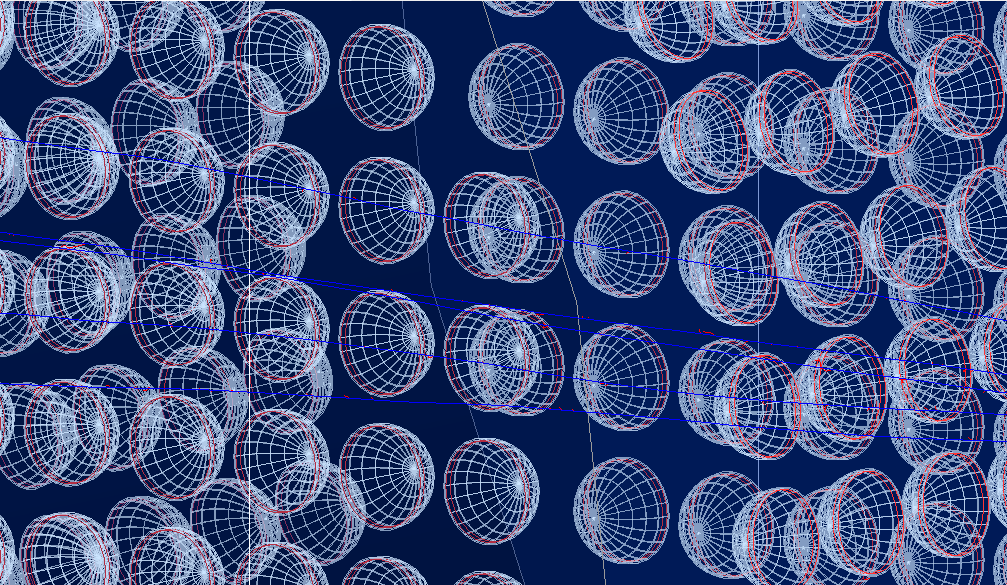
\includegraphics[width=0.82\textwidth]{../EvtDispl/Screenshot_from_2026-10-30_15-46-59.png}\caption{Event display 1.}\end{figure}
\begin{figure}[H]\centering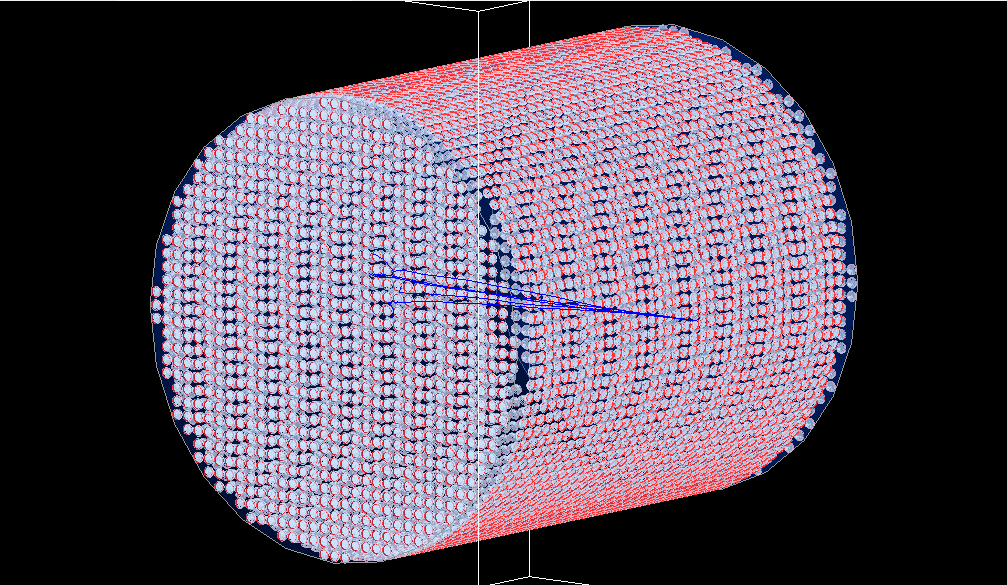
\includegraphics[width=0.82\textwidth]{../EvtDispl/Screenshot_from_2026-10-30_15-47-03.png}\caption{Event display 2.}\end{figure}
\begin{figure}[H]\centering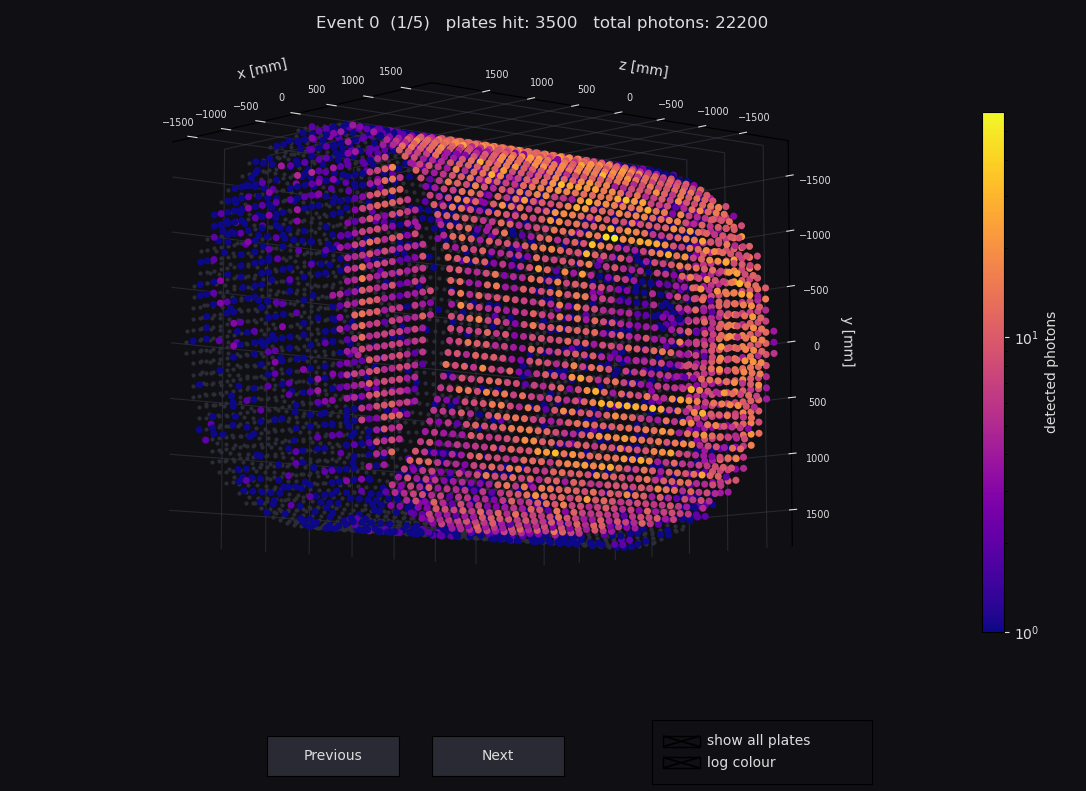
\includegraphics[width=0.82\textwidth]{../EvtDispl/Screenshot_from_2026-10-30_15-48-08.png}\caption{Event display 3.}\end{figure}
\begin{figure}[H]\centering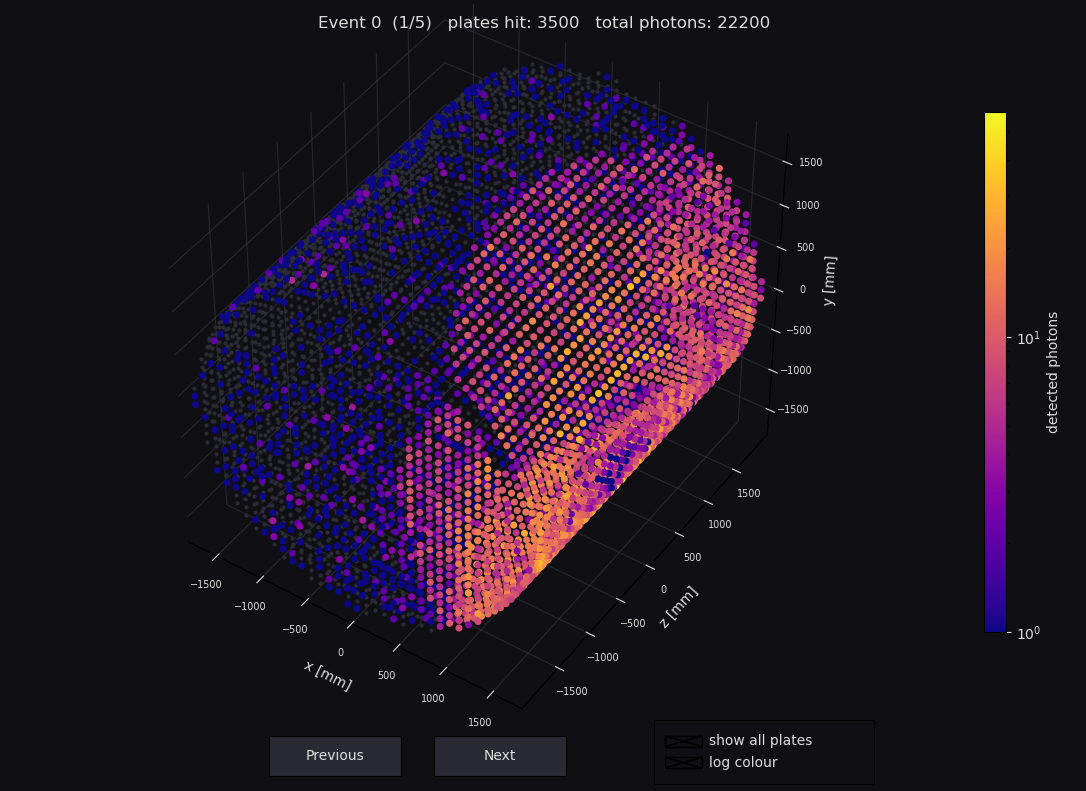
\includegraphics[width=0.82\textwidth]{../EvtDispl/Screenshot_from_2026-10-30_15-49-51.png}\caption{Event display 4.}\end{figure}
\begin{figure}[H]\centering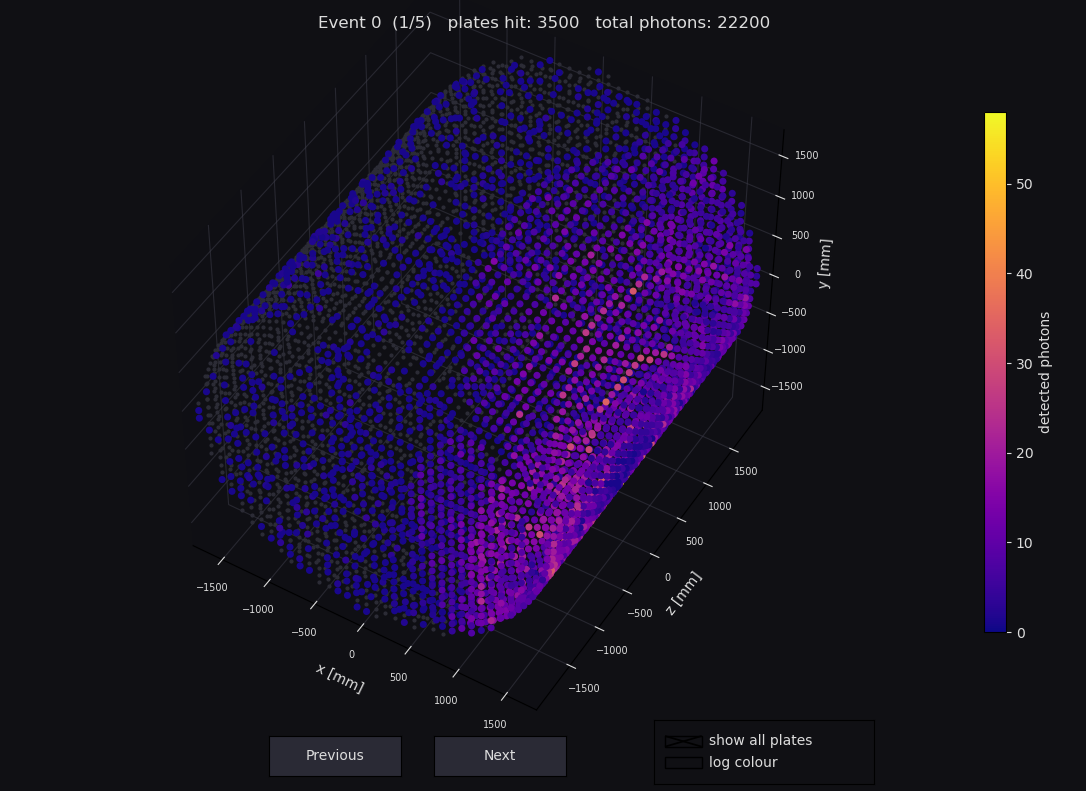
\includegraphics[width=0.82\textwidth]{../EvtDispl/Screenshot_from_2026-10-30_15-50-15.png}\caption{Event display 5.}\end{figure}

\subsection{Screenshoty (\texttt{Screenshots/})}
\begin{figure}[H]\centering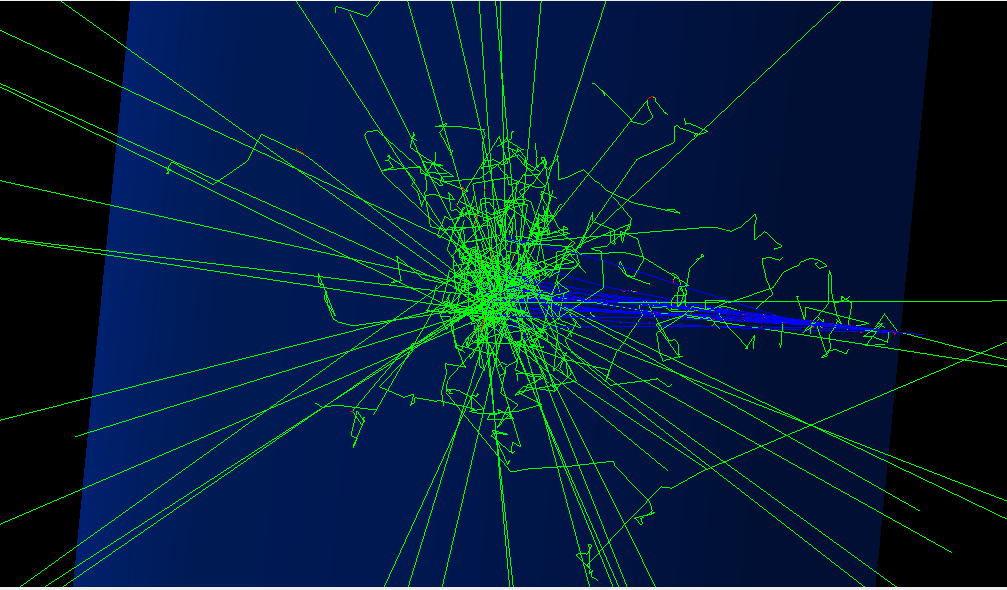
\includegraphics[width=0.82\textwidth]{../Screenshots/Screenshot_from_2026-10-24_15-01-46.png}\caption{Screenshot 1.}\end{figure}
\begin{figure}[H]\centering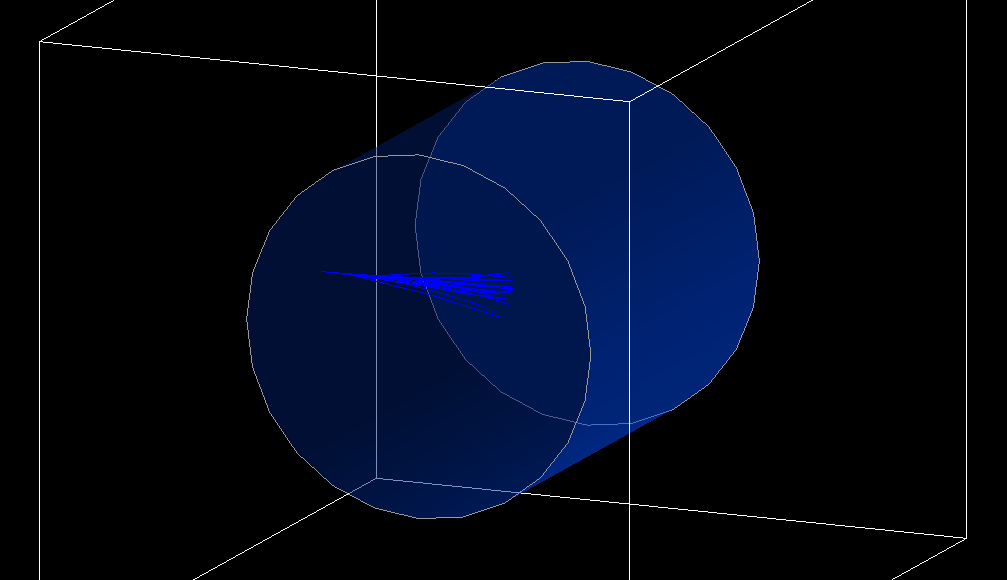
\includegraphics[width=0.82\textwidth]{../Screenshots/Screenshot_from_2026-10-24_15-11-40.png}\caption{Screenshot 2.}\end{figure}
\begin{figure}[H]\centering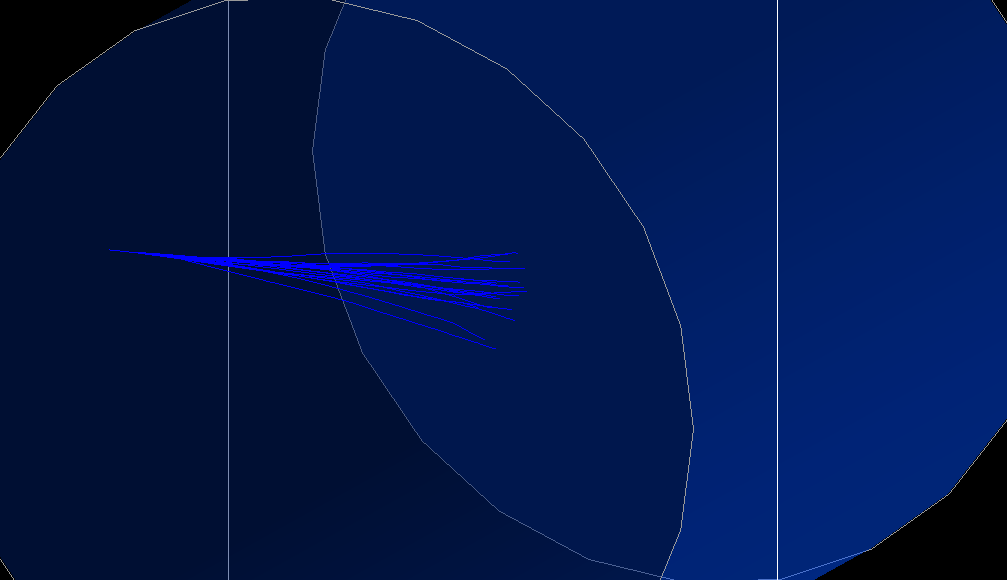
\includegraphics[width=0.82\textwidth]{../Screenshots/Screenshot_from_2026-10-24_15-11-45.png}\caption{Screenshot 3.}\end{figure}
\begin{figure}[H]\centering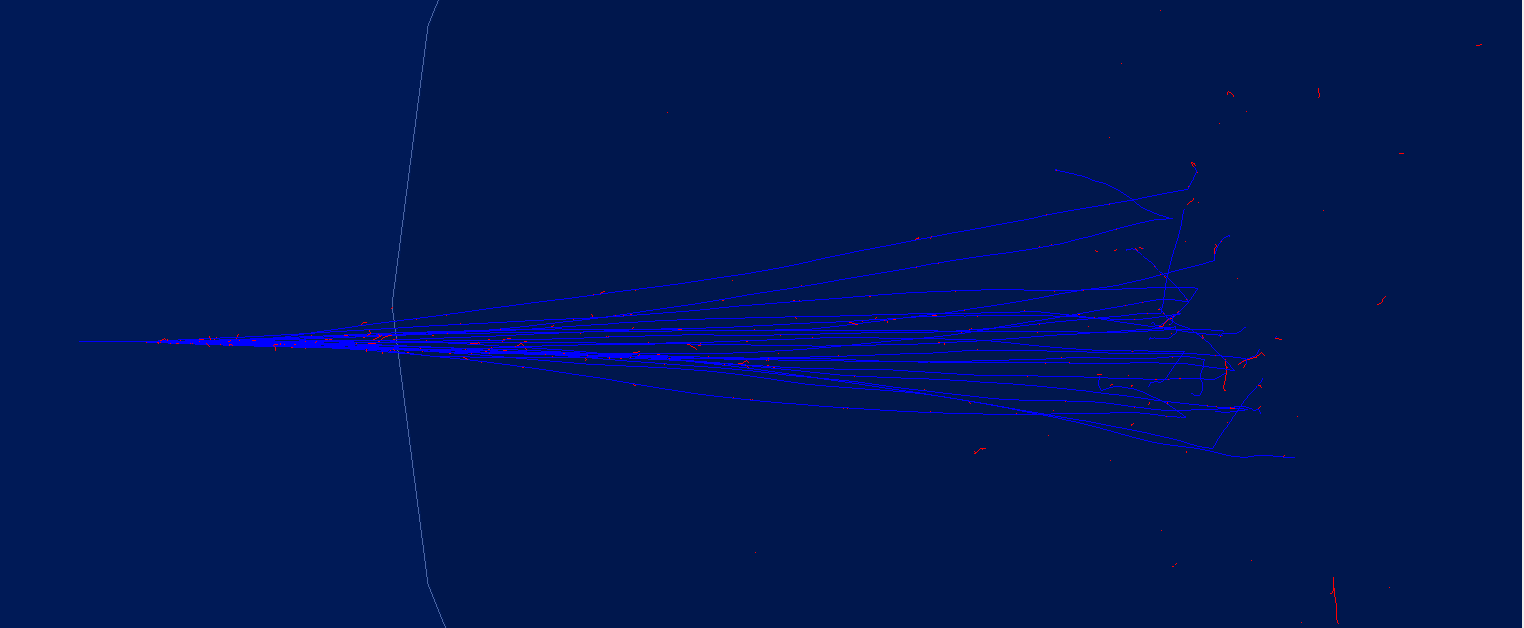
\includegraphics[width=0.82\textwidth]{../Screenshots/Screenshot_from_2026-10-25_11-50-18.png}\caption{Screenshot 4.}\end{figure}
\begin{figure}[H]\centering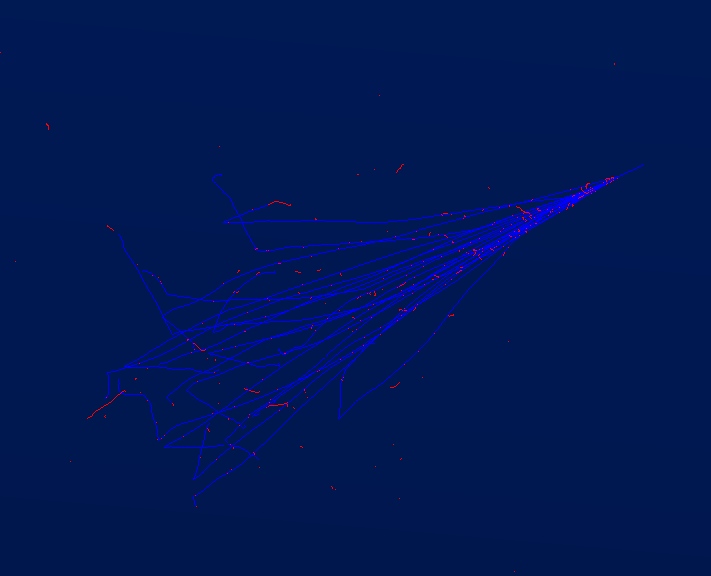
\includegraphics[width=0.82\textwidth]{../Screenshots/Screenshot_from_2026-10-25_11-50-39.png}\caption{Screenshot 5.}\end{figure}
\begin{figure}[H]\centering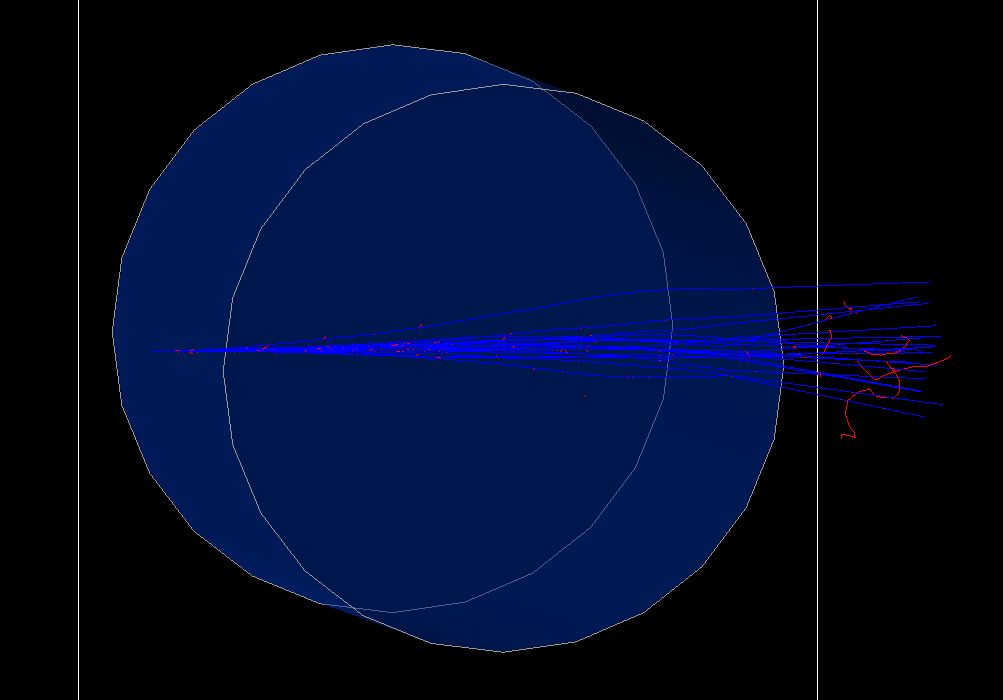
\includegraphics[width=0.82\textwidth]{../Screenshots/Screenshot_from_2026-10-25_11-52-45.png}\caption{Screenshot 6.}\end{figure}
\begin{figure}[H]\centering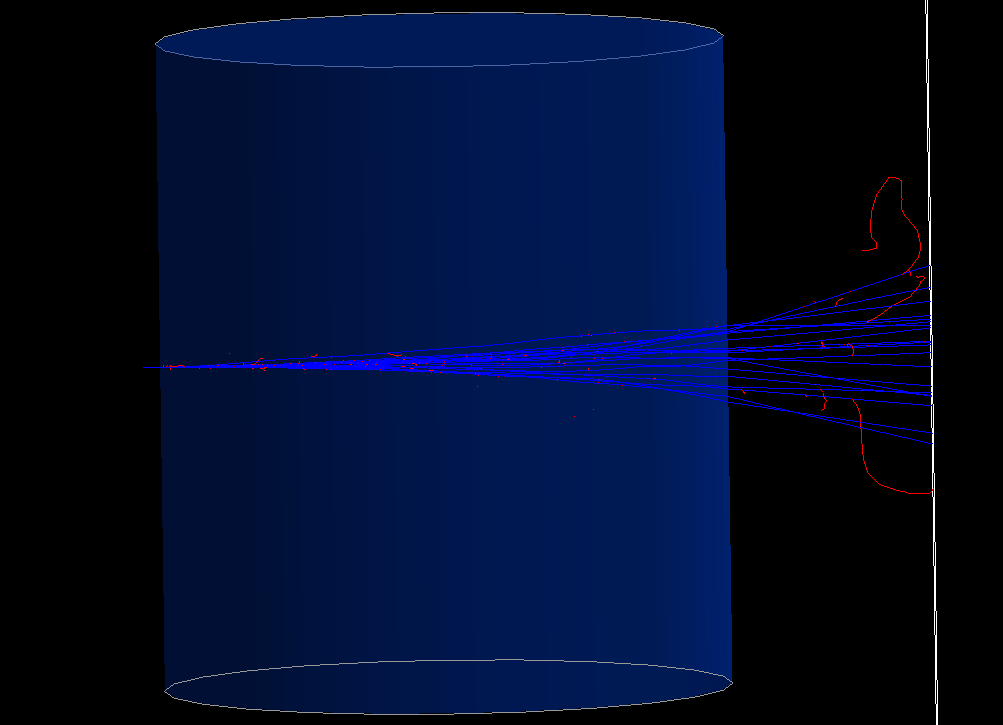
\includegraphics[width=0.82\textwidth]{../Screenshots/Screenshot_from_2026-10-25_11-53-16.png}\caption{Screenshot 7.}\end{figure}
\begin{figure}[H]\centering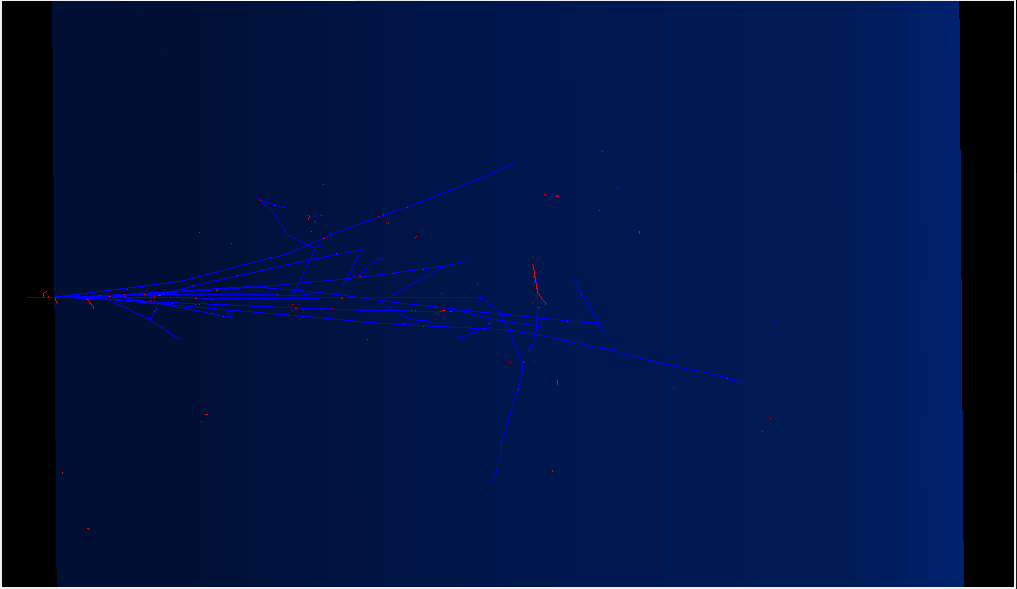
\includegraphics[width=0.82\textwidth]{../Screenshots/Screenshot_from_2026-10-30_09-00-12.png}\caption{Screenshot 8.}\end{figure}
\begin{figure}[H]\centering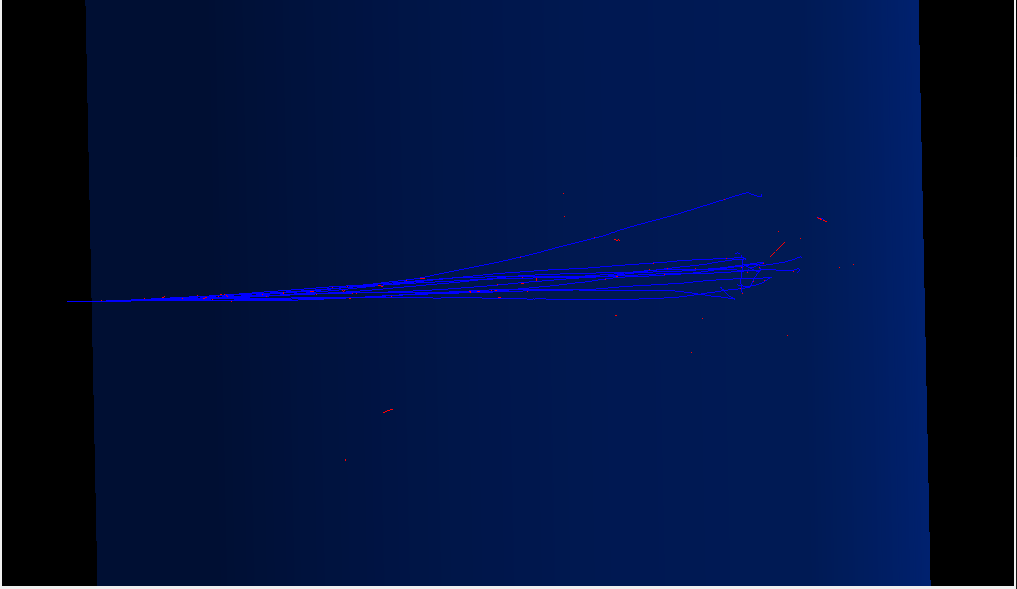
\includegraphics[width=0.82\textwidth]{../Screenshots/Screenshot_from_2026-10-30_09-00-46.png}\caption{Screenshot 9.}\end{figure}
\begin{figure}[H]\centering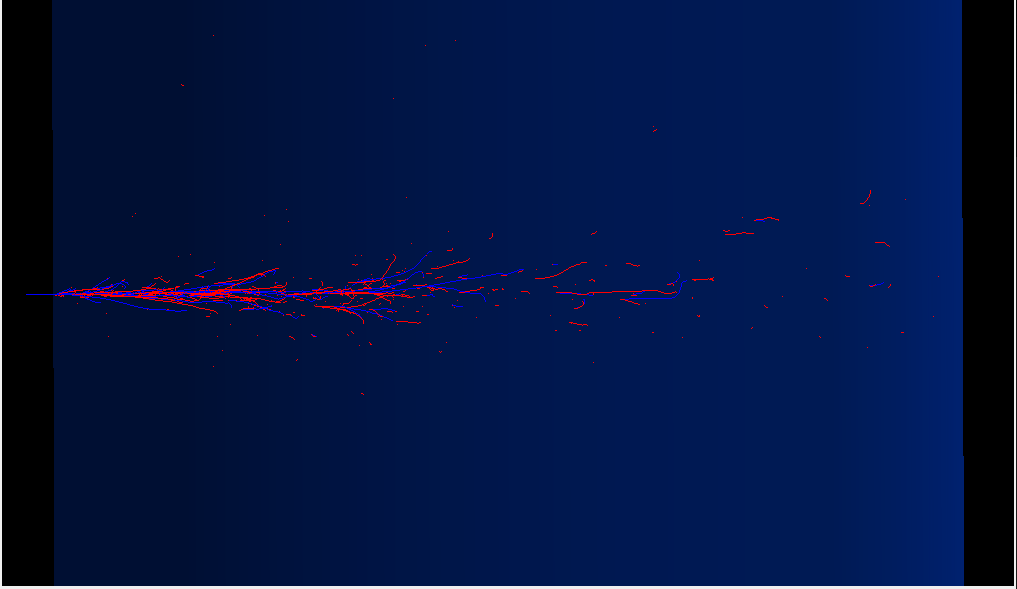
\includegraphics[width=0.82\textwidth]{../Screenshots/Screenshot_from_2026-10-30_09-01-35.png}\caption{Screenshot 10.}\end{figure}

\end{document}
